The Transverse Field Ising (TFI) Model is a well-studied spin lattice model that is often used to benchmark numerical methods. We introduce the TFI model in Section \ref{sec:TFI_model}. We then proceed by benchmarking disoTPS methods on the model. We first perform ground state searches using imaginary time evolution in Section \ref{sec:TFI_ground_state_search}. We benchmark the different proposed algorithms for the YB move and compare the first and second order TEBD algorithms. We further show numerical evidence that disoTPS are able to capture area law entanglement. Lastly we perform a ground state search on the honeycomb lattice, showing that disoTPS can be easily generalized to different lattice types. In Section \ref{sec:TFI_time_evolution} we perform a global quench and compute real time evolution. We observe that disoTPS struggles with the rapid entanglement growth and discuss some ideas for overcoming the problem. \par
We compare the results obtained with disoTPS to reference DMRG simulations using the tenpy library \cite{cite:tenpy}. The DMRG simulations are performed by "snaking" an MPS through the 2D lattice as shown in Figure \figref{fig:tenpy_snaking}. The disadvantage of this method is that sites that are close to each other in the lattice can be far apart in the MPS. Because of the close proximity of these sites we expect entanglement to build up between them. This entanglement cannot be captured well by the MPS because of its finite bond dimension, which is only able to capture entanglement locally in the MPS. We thus expect DMRG to break down for large systems. However, because of the low computational complexity of DMRG, one can scale the bond dimension to large values. For the lattice sizes we looked at this still allows for accurate results.
\begin{figure}
	\centering
	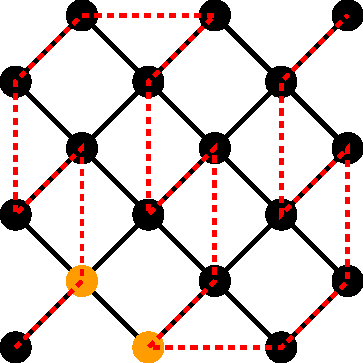
\includegraphics[scale=0.6]{figures/tikz/TFI/dmrg_snaking/dmrg_snaking.pdf}
	\caption{An MPS can be put on a 2D square lattice by "snaking" it through the lattice. The two sites marked in orange are nearest neighbour sites in the lattice, but are far apart in the MPS. Thus, entanglement between the two sites is hard to represent, requiring large bond dimensions.}
	\label{fig:tenpy_snaking}
\end{figure}

\section{The Transverse Field Ising Model}
\label{sec:TFI_model}
The Transverse Field Ising (TFI) model is a well-studied spin lattice model that is described by the Hamiltonian
\begin{equation}
	\label{eq:TFI_Hamiltonian}
	\hat{H}_\text{TFI} = -J\sum_{\langle i,j\rangle} \hat{\sigma}^x_i \hat{\sigma}^x_j - g\sum_{i} \hat{\sigma}^z_i,
\end{equation}
where $\langle i,j\rangle$ denotes pairs of nearest neighbours and $\hat{\sigma}^x_i, \hat{\sigma}^z_i$ are the Pauli matrices. The model is widely used for benchmarking numerical methods. Here we will only discuss the TFI model on a two-dimensional lattice, which can be mapped to a classical Ising model on a three-dimensional lattice \cite{cite:from_d_dimensional_quantum_to_dp1_dimensional_classical}. We will further restrict ourselves to the ferromagnetic case $J > 0$ and to zero temperature. In the limit of vanishing transverse field $g \rightarrow 0$ the model reduces to a classical 2D Ising model. The ground state is degenerate with all spins pointing either up or down in the $S^x$ direction. The associated phase is the classically disordered phase \cite{cite:critical_behavior_of_the_two_dim_ising_model_in_transverse_field, cite:quantum_ising_phases_and_transitions_in_transverse_ising_models}, or ferromagnetic phase. Taking the other limit, $g \gg J$, reduces the model to non-interacting spins in an external field. The ground state is unique with all spins pointing in $S^z$ direction. The corresponding phase is called the paramagnetic phase. There exists a quantum phase transition at a critical transverse field $g = g_\text{C}$ from the ferromagnetic to the paramagnetic phase. Blöte and Deng computed the value of the critical field for the TFI model on the square lattice as $g \approx 3.04438$ using Quantum Monte Carlo methods \cite{cite:cluster_monte_carlo_simulation_of_TFI}. \par
In the following we benchmark disoTPS methods on the TFI model. We first perform ground state searches using imaginary time evolution in section \ref{sec:TFI_ground_state_search}. We benchmark the different proposed algorithms for the YB move and compare the first and second order TEBD algorithms. We further show numerical evidence that disoTPS are able to capture area law entanglement. Lastly we perform a ground state search on the honeycomb lattice, showing that disoTPS is easily generalized to different lattice types. In seciont \ref{sec:TFI_time_evolution} we perform a global quench and compute real time evolution. We observe that disoTPS struggles with the rapid entanglement growth and discuss some ideas for overcoming the problem. \par
We compare the results obtained with disoTPS to reference DMRG simulations using the tenpy library \cite{cite:tenpy}. The DMRG simulations are performed by "snaking" an MPS through the 2D lattice as shown in figure \figref{fig:tenpy_snaking}. The disadvantage of this method is that sites that are close to each other in the lattice can be far apart in the MPS. Because of the close proximity of these sites we expect entanglement to build up between them. This entanglement cannot be captured well by the MPS because of its finite bond dimension, which is only able to capture entanglement locally in the MPS. We thus expect DMRG to break down for large systems. However, because of the low computational complexity of DMRG, one can scale the bond dimension to large values. For the lattice sizes we looked at this still allows for accurate results.
\begin{figure}
\centering
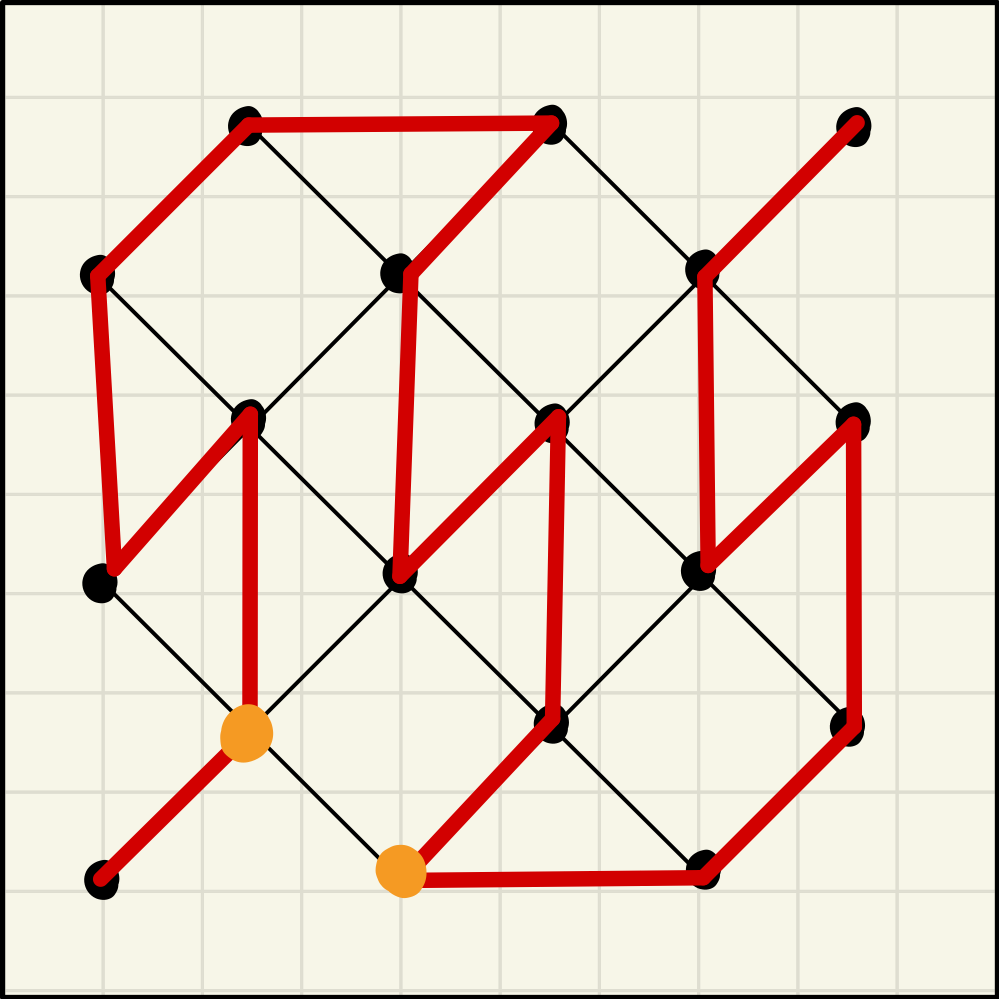
\includegraphics[width=0.4\textwidth]{figures/TFI/tenpy_snaking.jpeg}
\caption{An MPS can be put on a 2D square lattice by "snaking" it through the lattice. The two sites marked in orange are nearest neighbour sites in the lattice, but are far apart in the MPS. Thus, entanglement between the two sites is hard to represent, requiring large bond dimensions.}
\label{fig:tenpy_snaking}
\end{figure}


\section{Ground State Search}
\label{sec:TFI_ground_state_search}
\begin{figure}
	\centering
	\begin{minipage}{1.0\textwidth}
		\centering
		\begin{tikzpicture}[scale=1, trim axis left, trim axis right]
			\begin{axis}[ylabel={$\Delta E / E_\text{exact}$}, grid=both, grid style={gray!20}, every axis plot/.append style={very thick}, scale only axis, height=\gsEnergyVsDtauFigureHeight, width=\gsEnergyVsDtauFigureWidth, xmode=log, ymode=log, ymin=1e-6, ymax=1e-1, legend style={nodes={scale=\legendscale, transform shape, font=\small}}, legend pos=south west, title={\footnotesize\textbf{SVD}}, xticklabels={}, legend cell align={left}]
				%	
				\addplot[color = 3blue1, mark=*]
				table[x=dtau, y=delta_E_D_max_2, col sep=space]{figures/plots/TFI/gs_energy_vs_dtau/data/gs_energy_vs_dtau_square_svd.txt};
				\addlegendentry{$D = 2$}
				%	
				\addplot[color = 3blue2, mark=*]
				table[x=dtau, y=delta_E_D_max_4, col sep=space]{figures/plots/TFI/gs_energy_vs_dtau/data/gs_energy_vs_dtau_square_svd.txt};
				\addlegendentry{$D = 4$}
				%	
				\addplot[color = 3blue3, mark=*]
				table[x=dtau, y=delta_E_D_max_6, col sep=space]{figures/plots/TFI/gs_energy_vs_dtau/data/gs_energy_vs_dtau_square_svd.txt};
				\addlegendentry{$D = 6$}
			\end{axis}%
		\end{tikzpicture}%
		\,\,
		\begin{tikzpicture}[scale=1, trim axis left, trim axis right]
			\begin{axis}[grid=both, grid style={gray!20}, every axis plot/.append style={very thick}, scale only axis, height=\gsEnergyVsDtauFigureHeight, width=\gsEnergyVsDtauFigureWidth, xmode=log, ymode=log, ymin=1e-6, ymax=1e-1, yticklabels={}, title={\footnotesize\textbf{SVD + init}}, xticklabels={}]
				%	
				\addplot[color = 3blue1, mark=*]
				table[x=dtau, y=delta_E_D_max_2, col sep=space]{figures/plots/TFI/gs_energy_vs_dtau/data/gs_energy_vs_dtau_square_svd_init_polar.txt};
				%\addlegendentry{$D = 2$}
				%	
				\addplot[color = 3blue2, mark=*]
				table[x=dtau, y=delta_E_D_max_4, col sep=space]{figures/plots/TFI/gs_energy_vs_dtau/data/gs_energy_vs_dtau_square_svd_init_polar.txt};
				%\addlegendentry{$D = 4$}
				%	
				\addplot[color = 3blue3, mark=*]
				table[x=dtau, y=delta_E_D_max_6, col sep=space]{figures/plots/TFI/gs_energy_vs_dtau/data/gs_energy_vs_dtau_square_svd_init_polar.txt};
				%\addlegendentry{$D = 6$}
			\end{axis}%
		\end{tikzpicture}%
		\,\,
		\begin{tikzpicture}[scale=1, trim axis left, trim axis right]
			\begin{axis}[grid=both, grid style={gray!20}, every axis plot/.append style={very thick}, scale only axis, height=\gsEnergyVsDtauFigureHeight, width=\gsEnergyVsDtauFigureWidth, xmode=log, ymode=log, ymin=1e-6, ymax=1e-1, yticklabels={}, title={\footnotesize\textbf{EV trunc}}, xticklabels={}]
				%	
				\addplot[color = 3blue1, mark=*]
				table[x=dtau, y=delta_E_D_max_2, col sep=space]{figures/plots/TFI/gs_energy_vs_dtau/data/gs_energy_vs_dtau_square_iterate_polar.txt};
				%\addlegendentry{$D = 2$}
				%	
				\addplot[color = 3blue2, mark=*]
				table[x=dtau, y=delta_E_D_max_4, col sep=space]{figures/plots/TFI/gs_energy_vs_dtau/data/gs_energy_vs_dtau_square_iterate_polar.txt};
				%\addlegendentry{$D = 4$}
				%	
				\addplot[color = 3blue3, mark=*]
				table[x=dtau, y=delta_E_D_max_6, col sep=space]{figures/plots/TFI/gs_energy_vs_dtau/data/gs_energy_vs_dtau_square_iterate_polar.txt};
				%\addlegendentry{$D = 6$}
			\end{axis}%
		\end{tikzpicture}%
		\,\,
		\begin{tikzpicture}[scale=1, trim axis left, trim axis right]
			\begin{axis}[grid=both, grid style={gray!20}, every axis plot/.append style={very thick}, scale only axis, height=\gsEnergyVsDtauFigureHeight, width=\gsEnergyVsDtauFigureWidth, xmode=log, ymode=log, ymin=1e-6, ymax=1e-1, yticklabels={}, title={\footnotesize\textbf{EV Rényi-2}}, xticklabels={}]
				%	
				\addplot[color = 3blue1, mark=*]
				table[x=dtau, y=delta_E_D_max_2, col sep=space]{figures/plots/TFI/gs_energy_vs_dtau/data/gs_energy_vs_dtau_square_svd_disent_renyi_2.0_power_iteration.txt};
				%\addlegendentry{$D = 2$}
				%	
				\addplot[color = 3blue2, mark=*]
				table[x=dtau, y=delta_E_D_max_4, col sep=space]{figures/plots/TFI/gs_energy_vs_dtau/data/gs_energy_vs_dtau_square_svd_disent_renyi_2.0_power_iteration.txt};
				%\addlegendentry{$D = 4$}
				%	
				\addplot[color = 3blue3, mark=*]
				table[x=dtau, y=delta_E_D_max_6, col sep=space]{figures/plots/TFI/gs_energy_vs_dtau/data/gs_energy_vs_dtau_square_svd_disent_renyi_2.0_power_iteration.txt};
				%\addlegendentry{$D = 6$}
			\end{axis}%
		\end{tikzpicture}%
	\end{minipage}
	\begin{minipage}{1.0\textwidth}
		\centering%
		% ====================================================================================
		% 2nd line
		% ====================================================================================
		\begin{tikzpicture}[scale=1, trim axis left, trim axis right]
			\begin{axis}[ylabel={$\Delta E / E_\text{exact}$}, grid=both, grid style={gray!20}, every axis plot/.append style={very thick}, scale only axis, height=\gsEnergyVsDtauFigureHeight, width=\gsEnergyVsDtauFigureWidth, xmode=log, ymode=log, ymin=1e-6, ymax=1e-1, title={\footnotesize\textbf{CG trunc}}, xticklabels={}]
				%	
				\addplot[color = 3blue1, mark=*]
				table[x=dtau, y=delta_E_D_max_2, col sep=space]{figures/plots/TFI/gs_energy_vs_dtau/data/gs_energy_vs_dtau_square_svd_disent_trunc_error_cg.txt};
				%\addlegendentry{$D = 2$}
				%	
				\addplot[color = 3blue2, mark=*]
				table[x=dtau, y=delta_E_D_max_4, col sep=space]{figures/plots/TFI/gs_energy_vs_dtau/data/gs_energy_vs_dtau_square_svd_disent_trunc_error_cg.txt};
				%\addlegendentry{$D = 4$}
				%	
				\addplot[color = 3blue3, mark=*]
				table[x=dtau, y=delta_E_D_max_6, col sep=space]{figures/plots/TFI/gs_energy_vs_dtau/data/gs_energy_vs_dtau_square_svd_disent_trunc_error_cg.txt};
				%\addlegendentry{$D = 6$}
			\end{axis}%
		\end{tikzpicture}%
		\,\,
		\begin{tikzpicture}[scale=1, trim axis left, trim axis right]
			\begin{axis}[grid=both, grid style={gray!20}, every axis plot/.append style={very thick}, scale only axis, height=\gsEnergyVsDtauFigureHeight, width=\gsEnergyVsDtauFigureWidth, xmode=log, ymode=log, ymin=1e-6, ymax=1e-1, yticklabels={}, title={\footnotesize\textbf{approx CG trunc}}, xticklabels={}]
				%	
				\addplot[color = 3blue1, mark=*]
				table[x=dtau, y=delta_E_D_max_2, col sep=space]{figures/plots/TFI/gs_energy_vs_dtau/data/gs_energy_vs_dtau_square_svd_disent_trunc_error_approx_cg.txt};
				%\addlegendentry{$D = 2$}
				%	
				\addplot[color = 3blue2, mark=*]
				table[x=dtau, y=delta_E_D_max_4, col sep=space]{figures/plots/TFI/gs_energy_vs_dtau/data/gs_energy_vs_dtau_square_svd_disent_trunc_error_approx_cg.txt};
				%\addlegendentry{$D = 4$}
				%	
				\addplot[color = 3blue3, mark=*]
				table[x=dtau, y=delta_E_D_max_6, col sep=space]{figures/plots/TFI/gs_energy_vs_dtau/data/gs_energy_vs_dtau_square_svd_disent_trunc_error_approx_cg.txt};
				%\addlegendentry{$D = 6$}
			\end{axis}%
		\end{tikzpicture}%
		\,\,
		\begin{tikzpicture}[scale=1, trim axis left, trim axis right]
			\begin{axis}[grid=both, grid style={gray!20}, every axis plot/.append style={very thick}, scale only axis, height=\gsEnergyVsDtauFigureHeight, width=\gsEnergyVsDtauFigureWidth, xmode=log, ymode=log, ymin=1e-6, ymax=1e-1, yticklabels={}, title={\footnotesize\textbf{TRM trunc}}, xticklabels={}]
				%	
				\addplot[color = 3blue1, mark=*]
				table[x=dtau, y=delta_E_D_max_2, col sep=space]{figures/plots/TFI/gs_energy_vs_dtau/data/gs_energy_vs_dtau_square_svd_disent_trunc_error_trm.txt};
				%\addlegendentry{$D = 2$}
				%	
				\addplot[color = 3blue2, mark=*]
				table[x=dtau, y=delta_E_D_max_4, col sep=space]{figures/plots/TFI/gs_energy_vs_dtau/data/gs_energy_vs_dtau_square_svd_disent_trunc_error_trm.txt};
				%\addlegendentry{$D = 4$}
				%	
				\addplot[color = 3blue3, mark=*]
				table[x=dtau, y=delta_E_D_max_6, col sep=space]{figures/plots/TFI/gs_energy_vs_dtau/data/gs_energy_vs_dtau_square_svd_disent_trunc_error_trm.txt};
				%\addlegendentry{$D = 6$}
			\end{axis}%
		\end{tikzpicture}%
		\,\,
		\begin{tikzpicture}[scale=1, trim axis left, trim axis right]
			\begin{axis}[grid=both, grid style={gray!20}, every axis plot/.append style={very thick}, scale only axis, height=\gsEnergyVsDtauFigureHeight, width=\gsEnergyVsDtauFigureWidth, xmode=log, ymode=log, ymin=1e-6, ymax=1e-1, yticklabels={}, title={\footnotesize\textbf{approx TRM trunc}}, xticklabels={}]
				%	
				\addplot[color = 3blue1, mark=*]
				table[x=dtau, y=delta_E_D_max_2, col sep=space]{figures/plots/TFI/gs_energy_vs_dtau/data/gs_energy_vs_dtau_square_svd_disent_trunc_error_approx_trm.txt};
				%\addlegendentry{$D = 2$}
				%	
				\addplot[color = 3blue2, mark=*]
				table[x=dtau, y=delta_E_D_max_4, col sep=space]{figures/plots/TFI/gs_energy_vs_dtau/data/gs_energy_vs_dtau_square_svd_disent_trunc_error_approx_trm.txt};
				%\addlegendentry{$D = 4$}
				%	
				\addplot[color = 3blue3, mark=*]
				table[x=dtau, y=delta_E_D_max_6, col sep=space]{figures/plots/TFI/gs_energy_vs_dtau/data/gs_energy_vs_dtau_square_svd_disent_trunc_error_approx_trm.txt};
				%\addlegendentry{$D = 6$}
			\end{axis}%
		\end{tikzpicture}%
	\end{minipage}
	\begin{minipage}{1.0\textwidth}
		\centering%
		% ====================================================================================
		% 3rd line
		% ====================================================================================
		\begin{tikzpicture}[scale=1, trim axis left, trim axis right]
			\begin{axis}[xlabel=$\Delta\tau$, ylabel={$\Delta E / E_\text{exact}$}, grid=both, grid style={gray!20}, every axis plot/.append style={very thick}, scale only axis, height=\gsEnergyVsDtauFigureHeight, width=\gsEnergyVsDtauFigureWidth, xmode=log, ymode=log, ymin=1e-6, ymax=1e-1, title={\footnotesize\textbf{CG Rényi-0.5}}]
				%	
				\addplot[color = 3blue1, mark=*]
				table[x=dtau, y=delta_E_D_max_2, col sep=space]{figures/plots/TFI/gs_energy_vs_dtau/data/gs_energy_vs_dtau_square_svd_disent_renyi_0.5_cg.txt};
				%\addlegendentry{$D = 2$}
				%	
				\addplot[color = 3blue2, mark=*]
				table[x=dtau, y=delta_E_D_max_4, col sep=space]{figures/plots/TFI/gs_energy_vs_dtau/data/gs_energy_vs_dtau_square_svd_disent_renyi_0.5_cg.txt};
				%\addlegendentry{$D = 4$}
				%	
				\addplot[color = 3blue3, mark=*]
				table[x=dtau, y=delta_E_D_max_6, col sep=space]{figures/plots/TFI/gs_energy_vs_dtau/data/gs_energy_vs_dtau_square_svd_disent_renyi_0.5_cg.txt};
				%\addlegendentry{$D = 6$}
			\end{axis}%
		\end{tikzpicture}%
		\,\,
		\begin{tikzpicture}[scale=1, trim axis left, trim axis right]
			\begin{axis}[xlabel=$\Delta\tau$, grid=both, grid style={gray!20}, every axis plot/.append style={very thick}, scale only axis, height=\gsEnergyVsDtauFigureHeight, width=\gsEnergyVsDtauFigureWidth, xmode=log, ymode=log, ymin=1e-6, ymax=1e-1, yticklabels={}, title={\footnotesize\textbf{appr.\,CG\,Rényi-0.5}}]
				%	
				\addplot[color = 3blue1, mark=*]
				table[x=dtau, y=delta_E_D_max_2, col sep=space]{figures/plots/TFI/gs_energy_vs_dtau/data/gs_energy_vs_dtau_square_svd_disent_renyi_0.5_approx_cg.txt};
				%\addlegendentry{$D = 2$}
				%	
				\addplot[color = 3blue2, mark=*]
				table[x=dtau, y=delta_E_D_max_4, col sep=space]{figures/plots/TFI/gs_energy_vs_dtau/data/gs_energy_vs_dtau_square_svd_disent_renyi_0.5_approx_cg.txt};
				%\addlegendentry{$D = 4$}
				%	
				\addplot[color = 3blue3, mark=*]
				table[x=dtau, y=delta_E_D_max_6, col sep=space]{figures/plots/TFI/gs_energy_vs_dtau/data/gs_energy_vs_dtau_square_svd_disent_renyi_0.5_approx_cg.txt};
				%\addlegendentry{$D = 6$}
			\end{axis}%
		\end{tikzpicture}%
		\,\,
		\begin{tikzpicture}[scale=1, trim axis left, trim axis right]
			\begin{axis}[xlabel=$\Delta\tau$, grid=both, grid style={gray!20}, every axis plot/.append style={very thick}, scale only axis, height=\gsEnergyVsDtauFigureHeight, width=\gsEnergyVsDtauFigureWidth, xmode=log, ymode=log, ymin=1e-6, ymax=1e-1, yticklabels={}, title={\footnotesize\textbf{TRM\,Rényi-0.5}}]
				%	
				\addplot[color = 3blue1, mark=*]
				table[x=dtau, y=delta_E_D_max_2, col sep=space]{figures/plots/TFI/gs_energy_vs_dtau/data/gs_energy_vs_dtau_square_svd_disent_renyi_0.5_trm.txt};
				%\addlegendentry{$D = 2$}
				%	
				\addplot[color = 3blue2, mark=*]
				table[x=dtau, y=delta_E_D_max_4, col sep=space]{figures/plots/TFI/gs_energy_vs_dtau/data/gs_energy_vs_dtau_square_svd_disent_renyi_0.5_trm.txt};
				%\addlegendentry{$D = 4$}
				%	
				\addplot[color = 3blue3, mark=*]
				table[x=dtau, y=delta_E_D_max_6, col sep=space]{figures/plots/TFI/gs_energy_vs_dtau/data/gs_energy_vs_dtau_square_svd_disent_renyi_0.5_trm.txt};
				%\addlegendentry{$D = 6$}
			\end{axis}%
		\end{tikzpicture}%
		\,\,
		\begin{tikzpicture}[scale=1, trim axis left, trim axis right]
			\begin{axis}[xlabel=$\Delta\tau$, grid=both, grid style={gray!20}, every axis plot/.append style={very thick}, scale only axis, height=\gsEnergyVsDtauFigureHeight, width=\gsEnergyVsDtauFigureWidth, xmode=log, ymode=log, ymin=1e-6, ymax=1e-1, yticklabels={}, title={\footnotesize\textbf{appr.\,TRM\,Rényi-0.5}}]
				%	
				\addplot[color = 3blue1, mark=*]
				table[x=dtau, y=delta_E_D_max_2, col sep=space]{figures/plots/TFI/gs_energy_vs_dtau/data/gs_energy_vs_dtau_square_svd_disent_renyi_0.5_approx_trm.txt};
				%\addlegendentry{$D = 2$}
				%	
				\addplot[color = 3blue2, mark=*]
				table[x=dtau, y=delta_E_D_max_4, col sep=space]{figures/plots/TFI/gs_energy_vs_dtau/data/gs_energy_vs_dtau_square_svd_disent_renyi_0.5_approx_trm.txt};
				%\addlegendentry{$D = 4$}
				%	
				\addplot[color = 3blue3, mark=*]
				table[x=dtau, y=delta_E_D_max_6, col sep=space]{figures/plots/TFI/gs_energy_vs_dtau/data/gs_energy_vs_dtau_square_svd_disent_renyi_0.5_approx_trm.txt};
				%\addlegendentry{$D = 6$}
			\end{axis}%
		\end{tikzpicture}%
	\end{minipage}
	\caption{We benchmark the different implemented methods for the YB move on the TFI model on a $4\times4$ square lattice. The transverse field is set to $g = 3.5$. We compute the ground state energy with imaginary TEBD for different time step sizes $\Delta\tau$. First row: SVD splitting without disentangling, SVD splitting with a disentangling unitary initialized with an SVD as in \cite{cite:isometric_tensor_network_states_in_two_dimensions, cite:efficient_simulation_of_dynamics_in_two_dimensional_quantum_spin_systems}, Evenbly-Vidal minimization of the truncation error, and Evenbly-Vidal minimization of the Rényi-2 entropy. Second row: Disentangling with Riemannian optimization of the truncation error. Third row: Disentangling with Riemannian optimization of the  Rényi-1/2 entropy. All iterative methods were run for a maximum of $N_\text{iter} = 100$ iterations per YB move. The bond dimension of the orthogonality hypersurface was set to $\chi = 6\cdot D$.}
	\label{fig:tfi_gs_energy_vs_dtau_different_methods}
\end{figure}
\begin{figure}
	\centering
	\begin{minipage}{1.0\textwidth}
		\centering
		\begin{tikzpicture}[scale=1, trim axis left, trim axis right]
			\begin{axis}[xlabel=$\text{d}\tau$, ylabel={$\Delta E / E_\text{exact}$}, grid=both, grid style={gray!20}, every axis plot/.append style={very thick}, scale only axis, height=\gsEnergyVsDtauFigureHeight, width=\gsEnergyVsDtauFigureWidth, xmode=log, ymode=log, ymin=1e-6, ymax=1e-1, title={$N_\text{iters} = 1$}]
				%	
				\addplot[color = 3blue1, mark=*]
				table[x=dtau, y=delta_E_D_max_2, col sep=space]{figures/plots/TFI/gs_energy_vs_dtau/data/gs_energy_vs_dtau_square_svd_disent_renyi_0.5_approx_trm_N_iters_1.txt};
				%\addlegendentry{$D = 2$}
				%	
				\addplot[color = 3blue2, mark=*]
				table[x=dtau, y=delta_E_D_max_4, col sep=space]{figures/plots/TFI/gs_energy_vs_dtau/data/gs_energy_vs_dtau_square_svd_disent_renyi_0.5_approx_trm_N_iters_1.txt};
				%\addlegendentry{$D = 4$}
				%	
				\addplot[color = 3blue3, mark=*]
				table[x=dtau, y=delta_E_D_max_6, col sep=space]{figures/plots/TFI/gs_energy_vs_dtau/data/gs_energy_vs_dtau_square_svd_disent_renyi_0.5_approx_trm_N_iters_1.txt};
				%\addlegendentry{$D = 6$}
			\end{axis}%
		\end{tikzpicture}%
		\,\,
		\begin{tikzpicture}[scale=1, trim axis left, trim axis right]
			\begin{axis}[xlabel=$\text{d}\tau$, grid=both, grid style={gray!20}, every axis plot/.append style={very thick}, scale only axis, height=\gsEnergyVsDtauFigureHeight, width=\gsEnergyVsDtauFigureWidth, xmode=log, ymode=log, ymin=1e-6, ymax=1e-1, yticklabels={}, title={$N_\text{iters} = 10$}]
				%	
				\addplot[color = 3blue1, mark=*]
				table[x=dtau, y=delta_E_D_max_2, col sep=space]{figures/plots/TFI/gs_energy_vs_dtau/data/gs_energy_vs_dtau_square_svd_disent_renyi_0.5_approx_trm_N_iters_10.txt};
				%\addlegendentry{$D = 2$}
				%	
				\addplot[color = 3blue2, mark=*]
				table[x=dtau, y=delta_E_D_max_4, col sep=space]{figures/plots/TFI/gs_energy_vs_dtau/data/gs_energy_vs_dtau_square_svd_disent_renyi_0.5_approx_trm_N_iters_10.txt};
				%\addlegendentry{$D = 4$}
				%	
				\addplot[color = 3blue3, mark=*]
				table[x=dtau, y=delta_E_D_max_6, col sep=space]{figures/plots/TFI/gs_energy_vs_dtau/data/gs_energy_vs_dtau_square_svd_disent_renyi_0.5_approx_trm_N_iters_10.txt};
				%\addlegendentry{$D = 6$}
			\end{axis}%
		\end{tikzpicture}%
		\,\,
		\begin{tikzpicture}[scale=1, trim axis left, trim axis right]
			\begin{axis}[xlabel=$\text{d}\tau$, grid=both, grid style={gray!20}, every axis plot/.append style={very thick}, scale only axis, height=\gsEnergyVsDtauFigureHeight, width=\gsEnergyVsDtauFigureWidth, xmode=log, ymode=log, ymin=1e-6, ymax=1e-1, yticklabels={}, title={$N_\text{iters} = 50$}]
				%	
				\addplot[color = 3blue1, mark=*]
				table[x=dtau, y=delta_E_D_max_2, col sep=space]{figures/plots/TFI/gs_energy_vs_dtau/data/gs_energy_vs_dtau_square_svd_disent_renyi_0.5_approx_trm_N_iters_50.txt};
				%\addlegendentry{$D = 2$}
				%	
				\addplot[color = 3blue2, mark=*]
				table[x=dtau, y=delta_E_D_max_4, col sep=space]{figures/plots/TFI/gs_energy_vs_dtau/data/gs_energy_vs_dtau_square_svd_disent_renyi_0.5_approx_trm_N_iters_50.txt};
				%\addlegendentry{$D = 4$}
				%	
				\addplot[color = 3blue3, mark=*]
				table[x=dtau, y=delta_E_D_max_6, col sep=space]{figures/plots/TFI/gs_energy_vs_dtau/data/gs_energy_vs_dtau_square_svd_disent_renyi_0.5_approx_trm_N_iters_50.txt};
				%\addlegendentry{$D = 6$}
			\end{axis}%
		\end{tikzpicture}%
		\,\,
		\begin{tikzpicture}[scale=1, trim axis left, trim axis right]
			\begin{axis}[xlabel=$\text{d}\tau$, grid=both, grid style={gray!20}, every axis plot/.append style={very thick}, scale only axis, height=\gsEnergyVsDtauFigureHeight, width=\gsEnergyVsDtauFigureWidth, xmode=log, ymode=log, ymin=1e-6, ymax=1e-1, yticklabels={}, title={$N_\text{iters} = 200$}, legend style={nodes={scale=\legendscale, transform shape}}, legend pos=north west]
				%	
				\addplot[color = 3blue1, mark=*]
				table[x=dtau, y=delta_E_D_max_2, col sep=space]{figures/plots/TFI/gs_energy_vs_dtau/data/gs_energy_vs_dtau_square_svd_disent_renyi_0.5_approx_trm_N_iters_200.txt};
				\addlegendentry{$D = 2$}
				%	
				\addplot[color = 3blue2, mark=*]
				table[x=dtau, y=delta_E_D_max_4, col sep=space]{figures/plots/TFI/gs_energy_vs_dtau/data/gs_energy_vs_dtau_square_svd_disent_renyi_0.5_approx_trm_N_iters_200.txt};
				\addlegendentry{$D = 4$}
				%	
				\addplot[color = 3blue3, mark=*]
				table[x=dtau, y=delta_E_D_max_6, col sep=space]{figures/plots/TFI/gs_energy_vs_dtau/data/gs_energy_vs_dtau_square_svd_disent_renyi_0.5_approx_trm_N_iters_200.txt};
				\addlegendentry{$D = 6$}
			\end{axis}%
		\end{tikzpicture}%
	\end{minipage}
	\caption{In this figure we test how many iterations of Riemannian optimization are necessary for the approximate TRM algorithm minimizing the Rényi-$0.5$ entropy to converge. As a model we use the TFI model on a $4\times4$ suare lattice with a transverse field of $g = 3.5$. The bond dimension of the orthogonality hypersurface is set to $\chi=6\cdot D$. We compute the ground state energy with imaginary TEBD for different time step sizes $\text{d}\tau$.}
	\label{fig:tfi_gs_energy_vs_dtau_different_N_iters}
\end{figure}
\begin{figure}
	\centering
	\begin{tikzpicture}[scale=1, trim axis left, trim axis right]
		\begin{axis}[xlabel=$\text{d}\tau$, ylabel={$\Delta E / E_\text{exact}$}, grid=both, grid style={gray!20}, every axis plot/.append style={very thick}, scale only axis, height=\gsEnergyVsDtauFigureHeight, width=\gsEnergyVsDtauFigureWidth, xmode=log, ymode=log, ymin=1e-6, ymax=1e-1, title={TEBD1}]
			%	
			\addplot[color = 3blue1, mark=*]
			table[x=dtau, y=delta_E_D_max_2, col sep=space]{figures/plots/TFI/gs_energy_vs_dtau/data/gs_energy_vs_dtau_square_svd_disent_renyi_0.5_approx_trm_tebd1.txt};
			%\addlegendentry{$D = 2$}
			%	
			\addplot[color = 3blue2, mark=*]
			table[x=dtau, y=delta_E_D_max_4, col sep=space]{figures/plots/TFI/gs_energy_vs_dtau/data/gs_energy_vs_dtau_square_svd_disent_renyi_0.5_approx_trm_tebd1.txt};
			%\addlegendentry{$D = 4$}
			%	
			\addplot[color = 3blue3, mark=*]
			table[x=dtau, y=delta_E_D_max_6, col sep=space]{figures/plots/TFI/gs_energy_vs_dtau/data/gs_energy_vs_dtau_square_svd_disent_renyi_0.5_approx_trm_tebd1.txt};
			%\addlegendentry{$D = 6$}
		\end{axis}%
	\end{tikzpicture}%
	\,\,
	\begin{tikzpicture}[scale=1, trim axis left, trim axis right]
		\begin{axis}[xlabel=$\text{d}\tau$, grid=both, grid style={gray!20}, every axis plot/.append style={very thick}, scale only axis, height=\gsEnergyVsDtauFigureHeight, width=\gsEnergyVsDtauFigureWidth, xmode=log, ymode=log, ymin=1e-6, ymax=1e-1, yticklabels={}, title={TEBD2}, legend style={nodes={scale=\legendscale, transform shape}}]
			%	
			\addplot[color = 3blue1, mark=*]
			table[x=dtau, y=delta_E_D_max_2, col sep=space]{figures/plots/TFI/gs_energy_vs_dtau/data/gs_energy_vs_dtau_square_svd_disent_renyi_0.5_approx_trm_tebd2.txt};
			\addlegendentry{$D = 2$}
			%	
			\addplot[color = 3blue2, mark=*]
			table[x=dtau, y=delta_E_D_max_4, col sep=space]{figures/plots/TFI/gs_energy_vs_dtau/data/gs_energy_vs_dtau_square_svd_disent_renyi_0.5_approx_trm_tebd2.txt};
			\addlegendentry{$D = 4$}
			%	
			\addplot[color = 3blue3, mark=*]
			table[x=dtau, y=delta_E_D_max_6, col sep=space]{figures/plots/TFI/gs_energy_vs_dtau/data/gs_energy_vs_dtau_square_svd_disent_renyi_0.5_approx_trm_tebd2.txt};
			\addlegendentry{$D = 6$}
		\end{axis}%
	\end{tikzpicture}%
	\caption{\todo{Caption}}
	\label{fig:tfi_gs_energy_vs_dtau_TEBD1_vs_TEBD2}
\end{figure}
\begin{figure}
	\centering
	\begin{minipage}{1.0\textwidth}
		\centering
		\begin{tikzpicture}[scale=1, trim axis left, trim axis right]
			\begin{axis}[xlabel=$\Delta\tau$, ylabel={$\Delta E / E_\text{exact}$}, grid=both, grid style={gray!20}, every axis plot/.append style={very thick}, scale only axis, height=\gsEnergyVsDtauFigureHeight, width=\gsEnergyVsDtauFigureWidth, xmode=log, ymode=log, ymin=1e-6, ymax=1e-1, title={$D_\text{horizontal} = D$}]
				%	
				\addplot[color = 3blue1, mark=*]
				table[x=dtau, y=delta_E_D_max_2, col sep=space]{figures/plots/TFI/gs_energy_vs_dtau/data/gs_energy_vs_dtau_honeycomb_svd_disent_renyi_0.5_approx_trm_D_horizontal_equal_D.txt};
				%\addlegendentry{$D = 2$}
				%	
				\addplot[color = 3blue2, mark=*]
				table[x=dtau, y=delta_E_D_max_4, col sep=space]{figures/plots/TFI/gs_energy_vs_dtau/data/gs_energy_vs_dtau_honeycomb_svd_disent_renyi_0.5_approx_trm_D_horizontal_equal_D.txt};
				%\addlegendentry{$D = 4$}
				%	
				\addplot[color = 3blue3, mark=*]
				table[x=dtau, y=delta_E_D_max_6, col sep=space]{figures/plots/TFI/gs_energy_vs_dtau/data/gs_energy_vs_dtau_honeycomb_svd_disent_renyi_0.5_approx_trm_D_horizontal_equal_D.txt};
				%\addlegendentry{$D = 6$}
			\end{axis}%
		\end{tikzpicture}%
		\,\,
		\begin{tikzpicture}[scale=1, trim axis left, trim axis right]
			\begin{axis}[xlabel=$\Delta\tau$, grid=both, grid style={gray!20}, every axis plot/.append style={very thick}, scale only axis, height=\gsEnergyVsDtauFigureHeight, width=\gsEnergyVsDtauFigureWidth, xmode=log, ymode=log, ymin=1e-6, ymax=1e-1, yticklabels={}, title={$D_\text{horizontal} = D^2$}, legend style={nodes={scale=\legendscale, transform shape, font=\small}}]
				%	
				\addplot[color = 3blue1, mark=*]
				table[x=dtau, y=delta_E_D_max_2, col sep=space]{figures/plots/TFI/gs_energy_vs_dtau/data/gs_energy_vs_dtau_honeycomb_svd_disent_renyi_0.5_approx_trm_D_horizontal_equal_D_squared.txt};
				\addlegendentry{$D = 2$}
				%	
				\addplot[color = 3blue2, mark=*]
				table[x=dtau, y=delta_E_D_max_4, col sep=space]{figures/plots/TFI/gs_energy_vs_dtau/data/gs_energy_vs_dtau_honeycomb_svd_disent_renyi_0.5_approx_trm_D_horizontal_equal_D_squared.txt};
				\addlegendentry{$D = 4$}
				%	
				\addplot[color = 3blue3, mark=*]
				table[x=dtau, y=delta_E_D_max_6, col sep=space]{figures/plots/TFI/gs_energy_vs_dtau/data/gs_energy_vs_dtau_honeycomb_svd_disent_renyi_0.5_approx_trm_D_horizontal_equal_D_squared.txt};
				\addlegendentry{$D = 6$}
			\end{axis}%
		\end{tikzpicture}%
		\quad\quad
		\raisebox{15pt}
		{%
			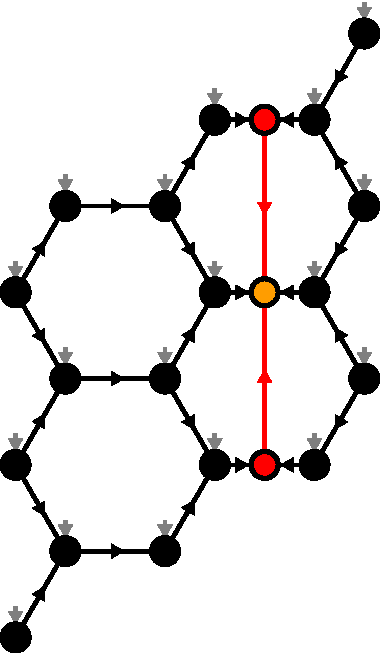
\includegraphics[scale=0.5]{figures/tikz/TFI/hexagonal_lattice/hexagonal_lattice_structure.pdf}
		}
	\end{minipage}
	\caption{In this figure we show imaginary TEBD results using disoTPS on the honeycomb lattice. We used two different values for the horizontal bond dimension, $D_\text{horizontal} = D$ and $D_\text{horizontal} = D^2$. The bond dimension along the orthogonality hypersurface was chosen as $\chi = 6\cdot D$. For the YB move we used the approximate Rényi-$0.5$ disentangler with a maximum of $N_\text{iter} = 100$ iterations per YB move. The model is the TFI model on a $4\times 4$ honeycomb lattice at a transverse field of $g = 3.5$. On the right we show the disoTPS structure of a $3\times 3$ honeycomb lattice as comparison.}
	\label{fig:tfi_gs_energy_vs_dtau_honeycomb}
\end{figure}
%\usetikzlibrary{backgrounds} % DEBUG
%background rectangle/.style={fill=olive!45}, show background rectangle
\begin{figure}
	\centering
	\begin{minipage}{1.0\textwidth}
		\hspace{280pt}
		\begin{tikzpicture}[scale=1, trim axis left, trim axis right]
			\begin{axis}[xlabel=$L$, ylabel={$E/N$}, grid=both, grid style={gray!20}, every axis plot/.append style={very thick}, scale only axis, height=\singleFigureHeight, width=\singleFigureWidth, ymin=-3.655, ymax=-3.565, legend style={at={(0.985,0.9)}, anchor=north east, font=\small, nodes={scale=\legendscale, transform shape}, label={[font=\small]above:{MPS DMRG}}}, legend columns=2, xmin=1, xmax=21, legend cell align={left}]
				%	
				\addplot[color = 7blue1]
				table[x=L, y=energy_density_tenpy_chi_16, col sep=space]{figures/plots/TFI/gs_search/data/gs_search_energy_density_vs_system_size.txt};
				\addlegendentry{$\chi = 16$}
				%
				\addplot[color = 7blue2]
				table[x=L, y=energy_density_tenpy_chi_32, col sep=space]{figures/plots/TFI/gs_search/data/gs_search_energy_density_vs_system_size.txt};
				\addlegendentry{$\chi = 32$}
				%
				\addplot[color = 7blue3]
				table[x=L, y=energy_density_tenpy_chi_64, col sep=space]{figures/plots/TFI/gs_search/data/gs_search_energy_density_vs_system_size.txt};
				\addlegendentry{$\chi = 64$}
				%
				\addplot[color = 7blue4]
				table[x=L, y=energy_density_tenpy_chi_128, col sep=space]{figures/plots/TFI/gs_search/data/gs_search_energy_density_vs_system_size.txt};
				\addlegendentry{$\chi = 128$}
				%
				\addplot[color = 7blue5]
				table[x=L, y=energy_density_tenpy_chi_256, col sep=space]{figures/plots/TFI/gs_search/data/gs_search_energy_density_vs_system_size.txt};
				\addlegendentry{$\chi = 256$}
				%
				\addplot[color = 7blue6]
				table[x=L, y=energy_density_tenpy_chi_512, col sep=space]{figures/plots/TFI/gs_search/data/gs_search_energy_density_vs_system_size.txt};
				\addlegendentry{$\chi = 512$}
				%
				\addplot[color = 7blue7]
				table[x=L, y=energy_density_tenpy_chi_1024, col sep=space]{figures/plots/TFI/gs_search/data/gs_search_energy_density_vs_system_size.txt};
				\addlegendentry{$\chi = 1024$}
				%
				\addplot[color = black]
				table[x=L, y=energy_density_tenpy_extrapolated, col sep=space]{figures/plots/TFI/gs_search/data/gs_search_energy_density_vs_system_size.txt};
				\addlegendentry{$\chi \rightarrow \infty$}
				%
			\end{axis}
			\begin{axis}[every axis plot/.append style={thick}, scale only axis, height=\singleFigureHeight, width=\singleFigureWidth, ymin=-3.655, ymax=-3.565, legend style={at={(0.42,0.9)}, anchor=north east, font=\small, nodes={scale=\legendscale, transform shape}, label={[font=\small]above:{YB-isoTPS}}}, legend columns=1, xmin=1, xmax=21, clip mode=individual, legend cell align={left}, yticklabels=\empty]
				%
				\addplot[color = 4red1, mark=*]
				table[x=L, y=energy_density_isoTPS_D_2, col sep=space]{figures/plots/TFI/gs_search/data/gs_search_energy_density_vs_system_size.txt};
				\addlegendentry{$D = 2$}
				%
				\addplot[color = 4red2, mark=*]
				table[x=L, y=energy_density_isoTPS_D_3, col sep=space]{figures/plots/TFI/gs_search/data/gs_search_energy_density_vs_system_size.txt};
				\addlegendentry{$D = 3$}
				%
				\addplot[color = 4red3, mark=*]
				table[x=L, y=energy_density_isoTPS_D_4, col sep=space]{figures/plots/TFI/gs_search/data/gs_search_energy_density_vs_system_size.txt};
				\addlegendentry{$D = 4$}
				%
				\addplot[color = 4red4, mark=*]
				table[x=L, y=energy_density_isoTPS_D_5, col sep=space]{figures/plots/TFI/gs_search/data/gs_search_energy_density_vs_system_size.txt};
				\addlegendentry{$D = 5$}
				%
				\draw[thick, black] (axis cs:16,-3.65) -- (axis cs:20,-3.65) -- (axis cs:20,-3.64) -- (axis cs:16,-3.64) -- (axis cs:16,-3.65);
				\draw[thick, black, dashed] (axis cs:20,-3.65) -- (\singleFigureWidth+20pt, \singleFigureHeight/2-\insetFigureHeight/2);
				\draw[thick, black, dashed] (axis cs:20,-3.64) -- (\singleFigureWidth+20pt, \singleFigureHeight/2+\insetFigureHeight/2);
			\end{axis}%
			\begin{axis}[xshift={\singleFigureWidth+20pt}, yshift={\singleFigureHeight/2-\insetFigureHeight/2}, grid=both, grid style={gray!20}, every axis plot/.append style={very thick}, scale only axis, height=\insetFigureHeight, width=\insetFigureWidth, ymin=-3.65, ymax=-3.64, xmin=16, xmax=20, clip marker paths=true, xtick={17,18,19}, ytick=\empty, xlabel=$L$]
				%	
				\addplot[color = 7blue1]
				table[x=L, y=energy_density_tenpy_chi_16, col sep=space]{figures/plots/TFI/gs_search/data/gs_search_energy_density_vs_system_size.txt};
				%\addlegendentry{$\chi = 16$}
				%
				\addplot[color = 7blue2]
				table[x=L, y=energy_density_tenpy_chi_32, col sep=space]{figures/plots/TFI/gs_search/data/gs_search_energy_density_vs_system_size.txt};
				%\addlegendentry{$\chi = 32$}
				%
				\addplot[color = 7blue3]
				table[x=L, y=energy_density_tenpy_chi_64, col sep=space]{figures/plots/TFI/gs_search/data/gs_search_energy_density_vs_system_size.txt};
				%\addlegendentry{$\chi = 64$}
				%
				\addplot[color = 7blue4]
				table[x=L, y=energy_density_tenpy_chi_128, col sep=space]{figures/plots/TFI/gs_search/data/gs_search_energy_density_vs_system_size.txt};
				%\addlegendentry{$\chi = 128$}
				%
				\addplot[color = 7blue5]
				table[x=L, y=energy_density_tenpy_chi_256, col sep=space]{figures/plots/TFI/gs_search/data/gs_search_energy_density_vs_system_size.txt};
				%\addlegendentry{$\chi = 256$}
				%
				\addplot[color = 7blue6]
				table[x=L, y=energy_density_tenpy_chi_512, col sep=space]{figures/plots/TFI/gs_search/data/gs_search_energy_density_vs_system_size.txt};
				%\addlegendentry{$\chi = 512$}
				%
				\addplot[color = 7blue7]
				table[x=L, y=energy_density_tenpy_chi_1024, col sep=space]{figures/plots/TFI/gs_search/data/gs_search_energy_density_vs_system_size.txt};
				%\addlegendentry{$\chi = 1024$}
				%
				\addplot[color = black]
				table[x=L, y=energy_density_tenpy_extrapolated, col sep=space]{figures/plots/TFI/gs_search/data/gs_search_energy_density_vs_system_size.txt};
				%\addlegendentry{$\chi \rightarrow \infty$}
				%
				%
				\addplot[color = 4red1, mark=*]
				table[x=L, y=energy_density_isoTPS_D_2, col sep=space]{figures/plots/TFI/gs_search/data/gs_search_energy_density_vs_system_size.txt};
				%\addlegendentry{$D = 2$}
				%
				\addplot[color = 4red2, mark=*]
				table[x=L, y=energy_density_isoTPS_D_3, col sep=space]{figures/plots/TFI/gs_search/data/gs_search_energy_density_vs_system_size.txt};
				%\addlegendentry{$D = 3$}
				%
				\addplot[color = 4red3, mark=*]
				table[x=L, y=energy_density_isoTPS_D_4, col sep=space]{figures/plots/TFI/gs_search/data/gs_search_energy_density_vs_system_size.txt};
				%\addlegendentry{$D = 4$}
				%
				\addplot[color = 4red4, mark=*]
				table[x=L, y=energy_density_isoTPS_D_5, col sep=space]{figures/plots/TFI/gs_search/data/gs_search_energy_density_vs_system_size.txt};
				%\addlegendentry{$D = 4$}
				%
			\end{axis}
		\end{tikzpicture}%
	\end{minipage}
	\caption{In this figure we plot the energy density $E/N$ of the TFI model against the linear system size $L$. The system is put on a diagonal $L\times L$ square lattice consisting of $N = 2L^2$ spins, at a transverse field $g = 3.5$. DMRG results are extrapolated to infinite bond dimension $\chi\rightarrow\infty$. The YB-isoTPS results were achieved with imaginary TEBD. For the YB move we used the approximate TRM Rényi-$0.5$ disentangler, which was run for a maximum of $N_\text{iter} = 100$ iterations per YB move. The maximum bond dimension of the orthogonality hypersurface was set to $\chi=6\cdot D$.}
	\label{fig:YB_isoTPS_gs_search_larger_systems}
\end{figure}
\begin{figure}
	\centering
	\hspace{260pt}
	\begin{tikzpicture}[scale=1, trim axis left, trim axis right]
		\centering
		\begin{axis}[xlabel=$L$, ylabel={$E/N$}, grid=both, grid style={gray!20}, every axis plot/.append style={very thick}, scale only axis, height=\singleFigureHeight, width=\singleFigureWidth, legend style={at={(0.985,0.02)}, anchor=south east, font=\small, nodes={scale=\legendscale, transform shape}, label={[font=\small]above:{MPS DMRG}}}, legend columns=2, xmin=1, xmax=21, legend cell align={left}, ymode=log, ymin=1e-6, ymax=1e-2]
			%	
			\addplot[color = 7blue1]
			table[x=L, y=error_tenpy_chi_16, col sep=space]{figures/plots/TFI/gs_search/data/gs_search_relative_energy_error_compared_to_extrapolated_DMRG.txt};
			\addlegendentry{$\chi = 16$}
			%
			\addplot[color = 7blue2]
			table[x=L, y=error_tenpy_chi_32, col sep=space]{figures/plots/TFI/gs_search/data/gs_search_relative_energy_error_compared_to_extrapolated_DMRG.txt};
			\addlegendentry{$\chi = 32$}
			%
			\addplot[color = 7blue3]
			table[x=L, y=error_tenpy_chi_64, col sep=space]{figures/plots/TFI/gs_search/data/gs_search_relative_energy_error_compared_to_extrapolated_DMRG.txt};
			\addlegendentry{$\chi = 64$}
			%
			\addplot[color = 7blue4]
			table[x=L, y=error_tenpy_chi_128, col sep=space]{figures/plots/TFI/gs_search/data/gs_search_relative_energy_error_compared_to_extrapolated_DMRG.txt};
			\addlegendentry{$\chi = 128$}
			%
			\addplot[color = 7blue5]
			table[x=L, y=error_tenpy_chi_256, col sep=space]{figures/plots/TFI/gs_search/data/gs_search_relative_energy_error_compared_to_extrapolated_DMRG.txt};
			\addlegendentry{$\chi = 256$}
			%
			\addplot[color = 7blue6]
			table[x=L, y=error_tenpy_chi_512, col sep=space]{figures/plots/TFI/gs_search/data/gs_search_relative_energy_error_compared_to_extrapolated_DMRG.txt};
			\addlegendentry{$\chi = 512$}
			%
			\addplot[color = 7blue7]
			table[x=L, y=error_tenpy_chi_1024, col sep=space]{figures/plots/TFI/gs_search/data/gs_search_relative_energy_error_compared_to_extrapolated_DMRG.txt};
			\addlegendentry{$\chi = 1024$}
			%
		\end{axis}
		\begin{axis}[every axis plot/.append style={thick}, scale only axis, height=\singleFigureHeight, width=\singleFigureWidth, legend style={at={(0.42,0.02)}, anchor=south east, font=\small, nodes={scale=\legendscale, transform shape}, label={[font=\small]above:{disoTPS}}}, legend columns=1, xmin=1, xmax=21, clip mode=individual, legend cell align={left}, ymode=log, ymin=1e-6, ymax=1e-2, yticklabels=\empty]
			%
			\addplot[color = 3red1, mark=*]
			table[x=L, y=error_isoTPS_D_2, col sep=space]{figures/plots/TFI/gs_search/data/gs_search_relative_energy_error_compared_to_extrapolated_DMRG.txt};
			\addlegendentry{$D = 2$}
			%
			\addplot[color = 3red2, mark=*]
			table[x=L, y=error_isoTPS_D_3, col sep=space]{figures/plots/TFI/gs_search/data/gs_search_relative_energy_error_compared_to_extrapolated_DMRG.txt};
			\addlegendentry{$D = 3$}
			%
			\addplot[color = 3red3, mark=*]
			table[x=L, y=error_isoTPS_D_4, col sep=space]{figures/plots/TFI/gs_search/data/gs_search_relative_energy_error_compared_to_extrapolated_DMRG.txt};
			\addlegendentry{$D = 4$}
			%
		\end{axis}%
	\end{tikzpicture}%
	\caption{\todo{Caption}}
	\label{fig:disoTPS_gs_search_larger_systems_log}
\end{figure}

\section{Time Evolution after a Global Quench}
\label{sec:TFI_time_evolution}
%\usetikzlibrary{backgrounds} % DEBUG
%background rectangle/.style={fill=olive!45}, show background rectangle
\begin{figure}
	\centering
	\begin{minipage}{1.0\textwidth}
		\centering
		\begin{tikzpicture}[scale=1, trim axis left, trim axis right]
			\begin{axis}[xlabel=$t$, ylabel={$\langle\hat{\sigma}_z\rangle$}, grid=both, grid style={gray!20}, every axis plot/.append style={very thick}, scale only axis, height=\singleFigureHeight, width=\singleFigureWidth, legend style={at={(1.2715,0.9)}, anchor=north west, font=\small, nodes={scale=\legendscale, transform shape}, label={[font=\small]above:{MPS DMRG}}}, legend columns=1, legend cell align={left}, xmin=-0.05, xmax=1.05, ymin=0.78, ymax=1.02]
				%
				\addplot[color = 7blue1]
				table[x=t_tenpy, y=sz_chi_16, col sep=space]{figures/plots/TFI/global_quench/data/global_quench_g_critical_tenpy.txt};
				\addlegendentry{$\chi = 16$}
				%
				\addplot[color = 7blue2]
				table[x=t_tenpy, y=sz_chi_32, col sep=space]{figures/plots/TFI/global_quench/data/global_quench_g_critical_tenpy.txt};
				\addlegendentry{$\chi = 32$}
				%
				\addplot[color = 7blue3]
				table[x=t_tenpy, y=sz_chi_64, col sep=space]{figures/plots/TFI/global_quench/data/global_quench_g_critical_tenpy.txt};
				\addlegendentry{$\chi = 64$}
				%
				\addplot[color = 7blue4]
				table[x=t_tenpy, y=sz_chi_128, col sep=space]{figures/plots/TFI/global_quench/data/global_quench_g_critical_tenpy.txt};
				\addlegendentry{$\chi = 128$}
				%
				\addplot[color = 7blue5]
				table[x=t_tenpy, y=sz_chi_256, col sep=space]{figures/plots/TFI/global_quench/data/global_quench_g_critical_tenpy.txt};
				\addlegendentry{$\chi = 256$}
				%
				\addplot[color = 7blue6]
				table[x=t_tenpy, y=sz_chi_512, col sep=space]{figures/plots/TFI/global_quench/data/global_quench_g_critical_tenpy.txt};
				\addlegendentry{$\chi = 512$}
				%
				\addplot[color = 7blue7]
				table[x=t_tenpy, y=sz_chi_1024, col sep=space]{figures/plots/TFI/global_quench/data/global_quench_g_critical_tenpy.txt};
				\addlegendentry{$\chi = 1024$}
				%
			\end{axis}
			\begin{axis}[every axis plot/.append style={thick}, scale only axis, height=\singleFigureHeight, width=\singleFigureWidth, legend style={at={(1.015,0.9)}, anchor=north west, font=\small, nodes={scale=\legendscale, transform shape}, label={[font=\small]above:{disoTPS}}}, legend columns=1, clip mode=individual, legend cell align={left}, yticklabels=\empty, xmin=-0.05, xmax=1.05, ymin=0.78, ymax=1.02]
				%
				\addplot[color = 5red1]
				table[x=t_disoTPS, y=sz_disoTPS_D_2, col sep=space]{figures/plots/TFI/global_quench/data/global_quench_g_critical_disoTPS.txt};
				\addlegendentry{$D = 2$}
				%
				\addplot[color = 5red2]
				table[x=t_disoTPS, y=sz_disoTPS_D_3, col sep=space]{figures/plots/TFI/global_quench/data/global_quench_g_critical_disoTPS.txt};
				\addlegendentry{$D = 3$}
				%
				\addplot[color = 5red3]
				table[x=t_disoTPS, y=sz_disoTPS_D_4, col sep=space]{figures/plots/TFI/global_quench/data/global_quench_g_critical_disoTPS.txt};
				\addlegendentry{$D = 4$}
				%
				\addplot[color = 5red4]
				table[x=t_disoTPS, y=sz_disoTPS_D_5, col sep=space]{figures/plots/TFI/global_quench/data/global_quench_g_critical_disoTPS.txt};
				\addlegendentry{$D = 5$}
				%
				\addplot[color = 5red5]
				table[x=t_disoTPS, y=sz_disoTPS_D_6, col sep=space]{figures/plots/TFI/global_quench/data/global_quench_g_critical_disoTPS.txt};
				\addlegendentry{$D = 6$}
				%
			\end{axis}%
		\end{tikzpicture}%
	\end{minipage}
	\caption{In this figure we show the time evolution of the $\langle\hat{\sigma}_z\rangle$ expectation value of a spin in the middle of the $8\times8$ diagonal square lattice, containing in total $N = 128$ spins. As a model we use the TFI model at critical field $g_\text{C}$. We compute the time evolution once with DMRG on a MPS and once with disoTPS with the parameters given in the text. We observe good agreement up to times of $t\approx 0.2$, when the two disoTPS results diverge from the DMRG reference simulation.}
	\label{fig:disoTPS_time_evolution_g_critical}
\end{figure}
As a second experiment we study the capabilities of disoTPS to perform real-time evolution. For this we perform a global quench by initializing the disoTPS to a product state, which we then evolve in time, measuring local expectation values. We start with an all-up-state $|\Psi\rangle = |\uparrow\rangle\otimes\cdots\otimes|\uparrow\rangle$ on the square lattice and evolve with the Hamiltonian of the TFI model at critical transverse field $g \approx 3.04438$. At the critical field the entanglement is expected to grow very quickly, making this a hard problem. For the disoTPS we choose bond dimensions of $D\in\left\{2, 3, 4, 5, 6\right\}$, $\chi = 6\cdot D$ and a step size of $\Delta t = 0.02$. We evolve up to time $t = 1.0$, requiring 50 full TEBD iterations. For the YB-move we used approximate TRM disentangling optimizing the Rényi $\alpha = 0.5$ entropy for a maximum number of $N_\text{iter}^\text{YB} = 100$ iterations. For the application of the TEBD bond operators we used a maximum of $N_\text{iters}^\text{bond-op} = 100$ iterations. For a comparison we used the time evolution algorithm from \cite{cite:time_evolving_a_mps_with_long_range_interactions} defined on MPS, which is able to perform time evolution in the presence of long range interactions and is implemented in tenpy \cite{cite:tenpy}. For this reference simulation we used bond dimensions ranging from $\chi = 16$ to $\chi= 1024$ and a time step of $\Delta t = 0.01$. We show the results in figure \figref{fig:disoTPS_time_evolution_g_critical}. We observe that disoTPS is in good agreement with the reference simulation up to a time of $t\approx0.2$, at which the expectation value diverges. This happens at earlier times for smaller bond dimensions $D$. We expect that this fast divergence is due to the accumulated error of the YB move. One could improve the method by applying a per-column variational optimization as done in isoTPS \cite{cite:isometric_tensor_network_states_in_two_dimensions, cite:efficient_simulation_of_dynamics_in_two_dimensional_quantum_spin_systems}, which was found to be essential for real-time evolution \cite{cite:efficient_simulation_of_dynamics_in_two_dimensional_quantum_spin_systems}, or by improving the YB move. \par
%\usetikzlibrary{backgrounds} % DEBUG
%background rectangle/.style={fill=olive!45}, show background rectangle
\begin{figure}
	\centering
	\begin{minipage}[t]{1.0\textwidth}
		\hspace{20pt}
		\begin{tikzpicture}[scale=1, trim axis left, trim axis right]
			\begin{axis}[xlabel=$t$, ylabel=$\langle\hat{\sigma}_z\rangle$, grid=both, grid style={gray!20}, every axis plot/.append style={very thick}, scale only axis, height=\globalQuenchLargeFieldFigureHeight, width=\globalQuenchLargeFieldFigureWidth, xmin=-0.05, xmax=1.05, ymin=-1.1, ymax=1.1, legend style={nodes={scale=\legendscale, transform shape, font=\small}}, legend pos=south east]
				%	
				\addplot[color = 5blue1]
				table[x=t_tenpy, y=sz_chi_16, col sep=space]{figures/plots/TFI/global_quench/data/global_quench_g_6.0_tenpy_site_index_4_4_0.txt};
				\addlegendentry{$\chi= 16$}
				%	
				\addplot[color = 5blue2]
				table[x=t_tenpy, y=sz_chi_32, col sep=space]{figures/plots/TFI/global_quench/data/global_quench_g_6.0_tenpy_site_index_4_4_0.txt};
				\addlegendentry{$\chi= 32$}
				%	
				\addplot[color = 5blue3]
				table[x=t_tenpy, y=sz_chi_64, col sep=space]{figures/plots/TFI/global_quench/data/global_quench_g_6.0_tenpy_site_index_4_4_0.txt};
				\addlegendentry{$\chi= 64$}
				%	
				\addplot[color = 5blue4]
				table[x=t_tenpy, y=sz_chi_128, col sep=space]{figures/plots/TFI/global_quench/data/global_quench_g_6.0_tenpy_site_index_4_4_0.txt};
				\addlegendentry{$\chi= 128$}
				%	
				\addplot[color = 5blue5]
				table[x=t_tenpy, y=sz_chi_256, col sep=space]{figures/plots/TFI/global_quench/data/global_quench_g_6.0_tenpy_site_index_4_4_0.txt};
				\addlegendentry{$\chi= 256$}
				%
			\end{axis}%
			\begin{axis}[scale only axis, height=\globalQuenchLargeFieldFigureHeight, width=\globalQuenchLargeFieldFigureWidth, every axis plot/.append style={very thick}, xmin=-0.05, xmax=1.05, ymin=-1.1, ymax=1.1, legend style={nodes={scale=\legendscale, transform shape, font=\small}}, legend pos=north west]
				%	
				\addplot[color = 3red1]
				table[x=t_disoTPS, y=sz_disoTPS_D_2, col sep=space]{figures/plots/TFI/global_quench/data/global_quench_g_6.0_disoTPS_site_index_4_4_0.txt};
				\addlegendentry{$D = 2$}
				%	
				\addplot[color = 3red2]
				table[x=t_disoTPS, y=sz_disoTPS_D_4, col sep=space]{figures/plots/TFI/global_quench/data/global_quench_g_6.0_disoTPS_site_index_4_4_0.txt};
				\addlegendentry{$D = 4$}
				%	
				\addplot[color = 3red3]
				table[x=t_disoTPS, y=sz_disoTPS_D_6, col sep=space]{figures/plots/TFI/global_quench/data/global_quench_g_6.0_disoTPS_site_index_4_4_0.txt};
				\addlegendentry{$D = 6$}
				%
			\end{axis}%
		\end{tikzpicture}%
		\quad
		\raisebox{34.2pt}
		{%
			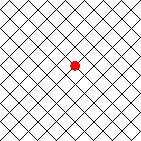
\includegraphics[scale=1.1]{figures/tikz/TFI/site_indices/site_index_a.pdf}
		}
	\end{minipage}	
	\par\medskip
	\begin{minipage}{1.0\textwidth}
		\hspace{20pt}
		\begin{tikzpicture}[scale=1, trim axis left, trim axis right]
			\begin{axis}[xlabel=$t$, ylabel=$\langle\hat{\sigma}_z\rangle$, grid=both, grid style={gray!20}, every axis plot/.append style={very thick}, scale only axis, height=\globalQuenchLargeFieldFigureHeight, width=\globalQuenchLargeFieldFigureWidth, xmin=-0.05, xmax=1.05, ymin=0.5, ymax=1.1]
				%	
				\addplot[color = 5blue1]
				table[x=t_tenpy, y=sz_chi_16, col sep=space]{figures/plots/TFI/global_quench/data/global_quench_g_6.0_tenpy_site_index_4_4_1.txt};
				%\addlegendentry{$\chi= 16$}
				%	
				\addplot[color = 5blue2]
				table[x=t_tenpy, y=sz_chi_32, col sep=space]{figures/plots/TFI/global_quench/data/global_quench_g_6.0_tenpy_site_index_4_4_1.txt};
				%\addlegendentry{$\chi= 32$}
				%	
				\addplot[color = 5blue3]
				table[x=t_tenpy, y=sz_chi_64, col sep=space]{figures/plots/TFI/global_quench/data/global_quench_g_6.0_tenpy_site_index_4_4_1.txt};
				%\addlegendentry{$\chi= 64$}
				%	
				\addplot[color = 5blue4]
				table[x=t_tenpy, y=sz_chi_128, col sep=space]{figures/plots/TFI/global_quench/data/global_quench_g_6.0_tenpy_site_index_4_4_1.txt};
				%\addlegendentry{$\chi= 128$}
				%	
				\addplot[color = 5blue5]
				table[x=t_tenpy, y=sz_chi_256, col sep=space]{figures/plots/TFI/global_quench/data/global_quench_g_6.0_tenpy_site_index_4_4_1.txt};
				%\addlegendentry{$\chi= 256$}
				%
			\end{axis}%
			\begin{axis}[scale only axis, height=\globalQuenchLargeFieldFigureHeight, width=\globalQuenchLargeFieldFigureWidth, every axis plot/.append style={very thick}, xmin=-0.05, xmax=1.05, ymin=0.5, ymax=1.1]
				%	
				\addplot[color = 3red1]
				table[x=t_disoTPS, y=sz_disoTPS_D_2, col sep=space]{figures/plots/TFI/global_quench/data/global_quench_g_6.0_disoTPS_site_index_4_4_1.txt};
				%\addlegendentry{$D = 2$}
				%	
				\addplot[color = 3red2]
				table[x=t_disoTPS, y=sz_disoTPS_D_4, col sep=space]{figures/plots/TFI/global_quench/data/global_quench_g_6.0_disoTPS_site_index_4_4_1.txt};
				%\addlegendentry{$D = 4$}
				%	
				\addplot[color = 3red3]
				table[x=t_disoTPS, y=sz_disoTPS_D_6, col sep=space]{figures/plots/TFI/global_quench/data/global_quench_g_6.0_disoTPS_site_index_4_4_1.txt};
				%\addlegendentry{$D = 5$}
				%
			\end{axis}%
		\end{tikzpicture}%
		\quad
		\raisebox{34.2pt}
		{%
			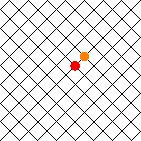
\includegraphics[scale=1.1]{figures/tikz/TFI/site_indices/site_index_b.pdf}
		}
	\end{minipage}
	\par\medskip
	\begin{minipage}{1.0\textwidth}
		\hspace{20pt}
		\begin{tikzpicture}[scale=1, trim axis left, trim axis right]
			\begin{axis}[xlabel=$t$, ylabel=$\langle\hat{\sigma}_z\rangle$, grid=both, grid style={gray!20}, every axis plot/.append style={very thick}, scale only axis, height=\globalQuenchLargeFieldFigureHeight, width=\globalQuenchLargeFieldFigureWidth, xmin=-0.05, xmax=1.05, ymin=0.9, ymax=1.05]
				%	
				\addplot[color = 5blue1]
				table[x=t_tenpy, y=sz_chi_16, col sep=space]{figures/plots/TFI/global_quench/data/global_quench_g_6.0_tenpy_site_index_5_5_0.txt};
				%\addlegendentry{$\chi= 16$}
				%	
				\addplot[color = 5blue2]
				table[x=t_tenpy, y=sz_chi_32, col sep=space]{figures/plots/TFI/global_quench/data/global_quench_g_6.0_tenpy_site_index_5_5_0.txt};
				%\addlegendentry{$\chi= 32$}
				%	
				\addplot[color = 5blue3]
				table[x=t_tenpy, y=sz_chi_64, col sep=space]{figures/plots/TFI/global_quench/data/global_quench_g_6.0_tenpy_site_index_5_5_0.txt};
				%\addlegendentry{$\chi= 64$}
				%	
				\addplot[color = 5blue4]
				table[x=t_tenpy, y=sz_chi_128, col sep=space]{figures/plots/TFI/global_quench/data/global_quench_g_6.0_tenpy_site_index_5_5_0.txt};
				%\addlegendentry{$\chi= 128$}
				%	
				\addplot[color = 5blue5]
				table[x=t_tenpy, y=sz_chi_256, col sep=space]{figures/plots/TFI/global_quench/data/global_quench_g_6.0_tenpy_site_index_5_5_0.txt};
				%\addlegendentry{$\chi= 256$}
				%
			\end{axis}%
			\begin{axis}[scale only axis, height=\globalQuenchLargeFieldFigureHeight, width=\globalQuenchLargeFieldFigureWidth, every axis plot/.append style={very thick}, xmin=-0.05, xmax=1.05, ymin=0.9, ymax=1.05]
				%	
				\addplot[color = 3red1]
				table[x=t_disoTPS, y=sz_disoTPS_D_2, col sep=space]{figures/plots/TFI/global_quench/data/global_quench_g_6.0_disoTPS_site_index_5_5_0.txt};
				%\addlegendentry{$D = 2$}
				%	
				\addplot[color = 3red2]
				table[x=t_disoTPS, y=sz_disoTPS_D_4, col sep=space]{figures/plots/TFI/global_quench/data/global_quench_g_6.0_disoTPS_site_index_5_5_0.txt};
				%\addlegendentry{$D = 4$}
				%	
				\addplot[color = 3red3]
				table[x=t_disoTPS, y=sz_disoTPS_D_6, col sep=space]{figures/plots/TFI/global_quench/data/global_quench_g_6.0_disoTPS_site_index_5_5_0.txt};
				%\addlegendentry{$D = 5$}
				%
			\end{axis}%
		\end{tikzpicture}%
		\quad
		\raisebox{34.2pt}
		{%
			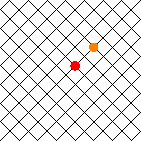
\includegraphics[scale=1.1]{figures/tikz/TFI/site_indices/site_index_c.pdf}
		}
	\end{minipage}
	\caption{In this figure we show the time evolution of the $\langle\hat{\sigma}_z\rangle$ expectation value of a spin in the middle of the lattice and its neighbouring spins. The position of the spins is visualized in the lattice next to the plots. As a model we use the TFI model in the paramagnetic phase with a transverse field of $g = 6$, put on an $8\times8$ diagonal square lattice containing in total $N = 128$ spins. We compute the time evolution once with DMRG on a MPS and once with disoTPS with the parameters given in the text.}
	\label{fig:disoTPS_time_evolution_g_6}
\end{figure}
Finally, we want to test the time evolution in a less challenging regime, for which we used the TFI model at a transverse field of $g = 6$, which is well in the paramagnetic phase. In this regime, entanglement is expected to build up much slower than when simulating at the critical field. We again initialize an all-up-state $|\Psi\rangle = |\uparrow\rangle\otimes\cdots\otimes|\uparrow\rangle$ on the $8\times8$ square lattice but additionally flip a spin in the center. We then compute the time evolution of the $\langle\hat{\sigma}_z\rangle$ expectation value of the flipped center spin and neighbouring spins. The results are shown in figure \figref{fig:disoTPS_time_evolution_g_6}. Note that the DMRG reference simulation converges for much lower bond dimensions $\chi$ compared to figure \figref{fig:disoTPS_time_evolution_g_critical}. We also observe much better agreement of disoTPS TEBD and MPS DMRG.